\documentclass[12pt]{article}

\usepackage[utf8]{inputenc} 
\usepackage[colorlinks=true]{hyperref} 
\usepackage[numbers, sort&compress]{natbib} 
\usepackage[]{geometry} 
\usepackage[]{amsmath} 
\usepackage[]{amsthm} 
\usepackage[]{bm} 
\usepackage[]{graphicx} 

% See: http://tex.stackexchange.com/a/3544
\renewcommand{\vec}[1]{\boldsymbol{\mathbf{#1}}}
\newcommand{\code}[1]{\texttt{#1}}

\bibliographystyle{plainnat}

\newtheorem{thm}{Theorem}

\theoremstyle{definition}
\newtheorem{defn}{Definition}

\setlength{\parskip}{\smallskipamount}

% Awful title.
\title{Markov's Monopoly}
\author{R.~Dougherty-Bliss}
\date{\today}

\begin{document}
\maketitle

\begin{abstract}
    We give historical background on Markov and the creation of his chains as
    they relate to the weak law of large numbers. We then provide a brief
    introduction to Markov chain analysis in the finite case. Chain theory is
    used to create a model of the boardgame Monopoly and a limiting
    distribution is given, with code available using the library Pykov.
\end{abstract}

\section{Introduction}
\label{sec:introduction}

Games of chance have long fascinated humans, often dictating large portions of
our lives. From letting a coin toss decide where to eat, to sitting at a
blackjack table, praying that the dealer busts, everyone has had experience
with these moments of chance. For Americans, there may be no game of chance
that has taken up more of our lives than the boardgame Monopoly.

Monopoly is a simple game conceived during the Great Depression. Players move
around a square board by rolling dice, purchasing iconic American property and
developing hotels on them as they go. The objective is ultimately bankrupt
other players; that is, to be the last player with any money. The main way to
affect the money of other players is to have them land on a property that you
own. If this happens, they must pay rent. The more hotels are built on a
property, the more expensive rent is. This creates a balancing act where
players must spend money purchasing and developing property to force other
players out, but must also maintain enough cash to ensure their own safety.
What would be beneficial is if there was someway to know a prior what the
``best'' spaces to develop were.

As it turns out, there is indeed a way to determine what the ``best'' spaces
are---if we quantify what we mean by ``best.'' The ``best'' spaces in Monopoly
are those that players are most likely to land on. Finding these spaces is a
problem that can be solved mathematically. As we will see in
Section~\ref{sec:monopoly_as_a_markov_chain}, Monopoly can be modeled as a
mathematical object known as a Markov chain. Markov chains are a very
well-understood tool from probability developed by the Russian mathematician
Markov in the early 20th century. As we will discuss in
Section~\ref{sec:introduction_to_markov_chains}, Markov chains model a specific
type of random behavior, and are applicable wherever this type of randomness
occurs. They have been used to model systems in physics, psychology, economics,
and various other applied fields \citep{bremaud1998markov}. They are
interesting in their own right, but we will explore the power they possess as
modeling tools, seeing first-hand why they have become mainstays of the
modeling world for a hundred years.

First we will discuss the origins of Markov chains in more detail.

\section{Markov in Context}
\label{sec:markov_in_context}

Though Markov chains are some of the most well-known and understood types of
stochastic processes, the background of their creation is often not discussed.
In Section~\ref{sec:origins_of_markov_chains} we will discuss the technical
goals of Markov chains, but here we will briefly describe Markov himself---the
mathematician behind the discovery.

Markov's life in Russia straddled the nineteenth and twentieth centuries. The
political climate of early twentieth-century Russia was tense, to say the
least. There was a revolution brewing that would change the world's political
landscape for decades to come. Despite this, there is little mention of
politics in the works of Markov. Theorems are not directly concerned with who
controls the government, so this is not surprising. However, the lack of
political commentary in Markov's work should not be taken as disinterest. By
the early twentieth-century Markov was an older, established academic. His
opinions were freely given---usually unsolicited. Markov wrote so many letters
of protest to newspapers that he was dubbed ``Andrew the Furious'' and ``the
militant academician'' \citep[p.~5]{basharin2004life}. In 1913 the Romanov
dynasty celebrated 300 years of rule over Russia. Being displeased with them,
Markov held a counter-celebration for 200 years of the Law of Large Numbers
\citep[chap.~10]{baclawski2008introduction}. In 1902 the ``socialist realist''
Russian writer Maxim Gorky was elected to the Russian Academy of Sciences. His
writings displayed a socialist viewpoint not in line with government position,
so his election was met with significant resistance. The Minister of Education
wrote that Gorky's election had a ``most distressing effect'' upon all
``right-thinking Russians,'' and ordered that it be withdrawn
\citep[p.~37]{yedlin1999maxim}. Markov protested this loudly and refused honors
from the tzar the following year\footnotemark. In 1912 the Russian Orthodox
Church excommunicated Leo Tolstoy. In response, Markov submitted a request to
the Church that he himself be excommunicated. The Church happily fulfilled this
request: ``[Markov] has seceded from God’s Church and [we] expunged him from
the lists of Orthodox believers'' \citep[p.~5]{basharin2004life}.

\footnotetext{Gorky was eventually reinstated to the Academy due to the efforts
of Markov and other prominent Russians.}

In his time as a student, graduate student, and eventually professor at the
St.~Petersburg school of mathematics, Markov studied under or collaborated with
many prominent Russian mathematicians. Markov's graduate advisor Chebyshev made
contributions to probability and number theory, proving the eponymous
Chebyshev's Inequality, which bounds the probability that a random variable can
fall certain distances away from its mean, and the Bertrand-Chebyshev Theorem,
which states that there exists a prime between $n$ and $2n$ for all integers $n
> 1$. Chebyshev's Inequality leads to a proof of the Weak Law of Large Numbers
(stated in Section~\ref{sec:origins_of_markov_chains}), and the
Bertrand-Chebyshev Theorem is an important step in discovering the distribution
of the primes, which will eventually lead mathematicians to the Riemann-Zeta
function, and thus to the famed Riemann Hypothesis. Lyapunov, slightly younger
than Markov, shared Chebyshev as an advisor. Lyapunov's thesis \emph{The
general problem of the stability of motion} introduced stability theory,
opening the doors to a rigorous study of dynamical systems. Among many other
things, Lyapunov applied his stability theory to show that movement of
particles in ``pear-shaped'' bodies of liquid was unstable, refuting an early
theory that the formation of orbital satellites, e.g. the Moon, was due to
rotating bodies of liquid \citep[pg.~276]{parks1992lyapunov}. In short, Markov
was surrounded by groundbreaking mathematicians. Interactions with his
contemporaries will prove crucial to Markov's own groundbreaking work.

True to his character, the interactions that spurred Markov's work were not the
pleasant collaborations---they were the drawn out, public arguments with
mathematicians outside of St.~Petersburg. A notable case of this is the tension
between the schools of mathematics of St.~Petersburg and Moscow. Many
mathematicians in the Moscow school were members of the Orthodox Church, and
used their research to argue for the validity of the Judeo-Christian concept of
``free will'' \citep[p.~255]{seneta1996markov}. Chuprov wrote that ``[t]he
`Moscow School' decidedly insists that free will is the \emph{conditio sine qua
non} of statistical laws governing everyday life''
\citep[p.~257]{seneta1996markov}. The St.~Petersburg school, and Markov in
particular, did not agree.

Markov and the Moscovian mathematician Nekrasov were the most prominent figures
in the bickering between the St.~Petersburg and Moscow schools. In many ways,
there were similar. Both outspoken, both established mathematicians, and they
both hated each other. Chuprov published a book that mentioned Nekrasov in a
positive light. Markov told Chuprov that Nekrasov's work was an ``abuse of
mathematics'' \citep[p.~257]{seneta1996markov}. Nekrasov published a paper on
probability that contained no proofs, and dedicated it to Chebyshev. Markov
took great offense to his advisor even being mentioned in a work without proof,
and one of many lengthy disputes between Nekrasov and Markov began. Out of the
Moscow school, Nekrasov was the most adamant in applying probability and
statistics to his Orthodox faith. Markov often worked to specifically refute
these points. In fact, as we shall soon see, Markov's study of his chains was
initiated almost entirely to provide a counterexample to a claim by Nekrasov
about the ``logical underpinnings'' of the Weak Law of Large Numbers.

\section{Origins of Markov Chains}
\label{sec:origins_of_markov_chains}

Despite their wide use in modeling today, Markov chains were not invented as
modeling techniques. They were invented primarily as a counterexample to claims
Nekrasov made about independence in the Weak Law of Large Numbers. We will take
the liberty to describe these claims in detail.

The Weak Law of Large Numbers (WLLN) is the formalization of a simple
intuition: if we draw a large enough sample from a distribution, then the
average value of the sample will approach the mean of the distribution. More
accurately, the probability that the average value will be far away from the
mean approaches zero as the sample size grows.

\begin{thm}[Weak Law of Large Numbers]
    \label{thm:WLLN}
    Let $X_1, X_2, \dots$ be an infinite sequence of independent and
    identically distributed (iid) random variables with finite expectation
    $E[X]$. Define the random variable $$\bar{X}_n := \frac{1}{n} \sum_{k =
    1}^n X_n$$ to be the ``mean'' of the first $n$ variables in the
    sequence. Then, $\bar{X}_n$ converges in probability to $E[X]$. That is,
    $$\lim_{n \to \infty} P(|\bar{X}_n - E[X]| < \epsilon) = 1$$ for all
    $\epsilon > 0$.
\end{thm}

As stated, this theorem applies to sequences of \emph{independent} variables.
Nekrasov noticed that the WLLN held if this condition was relaxed so that the
variables were only \emph{pairwise independent}. This was an interesting
result, but Nekrasov had larger designs. He believed that this pairwise
independence was implied by the philosophical concept of free will. He
concluded that the fact that average measurements in the ``real world'' seemed
to follow the WLLN implied that pairwise independence was a \emph{necessary}
condition for the WLLN to hold. That is, if $\bar{X}_n$ converges in
probability to $E[X]$ for some sequence $X_1, X_2, \dots$, then the sequence
must be pairwise independent. It is this claim that Markov set out to disprove
with his chains \citep{seneta1996markov}.

% Detail Markov's construction and an outline of his proof?

As a counterexample to Nekrasov's claims, Markov invented a special class of
discrete stochastic processes that satisfies the consequence of the WLLN with
dependent random variables. Today, this construction would be called a finite
Markov chain with positive transition probabilities. In addition to creating a
tidy counterexample, in a single paper Markov creates a new subfield of
probability.

\section{Introduction to Markov Chains}
\label{sec:introduction_to_markov_chains}

Informally, the Markov chains that we will consider are collections of states
equipped with probabilities of transitioning from one state to the other. To
describe them formally, we must make use of stochastic processes.

A discrete time stochastic process is a collection of random variables
$\{X_n\}$, $n = 0, 1, 2, \dots$, where each random variable $X_n$ is discrete
and takes values in a common, countable set, called the state space. We will
generally assume that the state space is $\{1, 2, 3, \dots\}$, but the
particular set is not important. We can think of the indexing variable $n$ as
``time'' and the value $X_n$ as the current state of the process at time $n$.
The distribution of the random variable $X_n$ completely describes the process
at time $n$ from a stochastic perspective. Thus, a discrete stochastic process
is a collection of states and random variables that describe the distribution
of the states of the process at any given time.

A simple example of a discrete stochastic process is the (infinite) random
walk. Suppose that we begin at a state labeled $0$ and flip a coin. If the coin
is heads, then we move to state $1$. If it is tails, then we move to state
$-1$. We continue this in an indefinitely, where our position at time $n$ is
given by the random variable $X_n$.

In the random walk example, the state of the process at time $n$ only depends
on the state of the process at time $n - 1$. To determine the possible states
at time $n$, we only need to know what state we were in at time $n - 1$, so we
can flip our coin. This property is called the Markov property, and will
characterize Markov chains.

\begin{defn}
    \label{defn:markov-prop}
    A discrete time stochastic process $\{X_n\}$ has the \emph{Markov property}
    iff $$P(X_n = i_n \mid X_0 = i_0, \dots, X_{n - 1} = i_{n - 1}) = P(X_n =
    i_n \mid X_{n - 1} = i_{n - 1})$$ for all sequences of states $\{i_k\}_{k =
    1}^n$. Any discrete time stochastic process that satisfies the Markov
    property is called a \emph{Markov chain}.
\end{defn}

Every Markov chain possesses a set of probabilities that describe the
probability of transitioning to state $i$ from state $j$ at time $n$. These are
called \emph{transition probabilities} and are denoted $$p_{ij}(n) = P(X_{n +
1} = i \mid X_n = j).$$ We will consider the case where the transition
probabilities are \emph{stationary}, or do not depend on $n$.

\begin{defn}
    \label{defn:trans-prob}
    If the transition probabilities are independent of $n$, that is, if
    $p_{ij}(n) = p_{ij}(n')$ for all times $n$ and $n'$, then they are called
    \emph{stationary}, \emph{time homogeneous}, or \emph{homogeneous}. In this
    case, the chain is called time homogeneous as well. The stationary
    transition probabilities are denoted $p_{ij}$. That is, $p_{ij}$ is the
    probability of moving to state $i$ from state $j$ at any time.
\end{defn}

From here, by ``Markov chain'' we mean ``time homogenous Markov chain,'' unless
noted otherwise.

Given a Markov chain, we can form a matrix of its transition probabilities.
This matrix is the defining aspect of a Markov chain.

\begin{defn}
    \label{defn:trans-matrix}
    The matrix
    $$P =
    \begin{bmatrix}
        p_{11} & p_{12} & p_{13} & \cdots \\
        p_{21} & p_{12} & p_{23} & \cdots \\
        \vdots & \vdots & \vdots
    \end{bmatrix}$$
    is the \emph{transition matrix} of a Markov chain. This matrix is
    \emph{stochastic} in that its columns sum to one. (It is certain that we
    will always transition to a state.) Conversely, any stochastic square
    matrix defines a Markov chain.
\end{defn}

Every transition matrix can be thought of as an adjacency matrix for a directed
graph. Thus, Markov chains can be represented as directed graphs with weighted
edges. An example for the matrix $$P =
\begin{bmatrix}
    0   & 0.1 & 0 & 0.4 \\
    0.6 & 0.9 & 0.3 & 0 \\
    0.4 & 0   & 0 & 0 \\
    0   & 0   & 0.7 & 0.6
\end{bmatrix}
$$
is shown in Figure~\ref{fig:graph}.

\begin{figure}[]
    \centering
    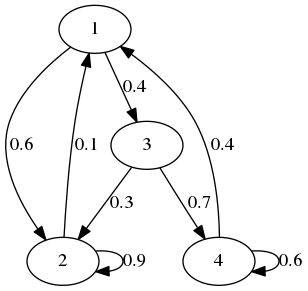
\includegraphics[width=.5\textwidth, keepaspectratio]{markov.png}
    \caption{Graphic representation of a Markov chain. Each directed edge $j
    \to i$ is labeled with the transition probability $p_{ij}$.}
    \label{fig:graph}
\end{figure}

We have discussed the one-step transition probabilities $p_{ij}$. The next
definition considers multiple steps. That is, we consider the probability that
we will transition to state $i$ from state $j$ in $n$ steps as opposed to one
step.

\begin{defn}
    \label{defn:n-step}
    The $n$-step transition probabilities are defined as $$p^{(n)}_{ij} = P(X_n
    = i \mid X_0 = j).$$ Thus, $p^{(n)}_{ij}$ is the probability of moving to
    state $i$ from state $j$ in $n$ steps. The matrix of $n$-step transition
    probabilities is denoted $P^{(n)}$.
\end{defn}

There is a connection between the transition matrix and the $n$-step transition
probabilities, namely that the matrix of $n$-step transition probabilities is
the transition matrix $P$ raised to the $n$th power.

\begin{thm}
    \label{thm:n-step-power}
    The $n$-step transition matrix $P^{(n)}$ is the transition matrix raised to
    the $n$th power. That is, $$P^{(n)} = P^n.$$
\end{thm}

Given an initial distribution of states $\vec{p}(0)$, the probability
distribution at time $n$ is simply $$\vec{p}(n) = P^n \vec{p}(0).$$ By the
long-term behavior of a Markov chain, we generally mean the behavior of
$\vec{p}(n)$ as $n$ tends to infinity. This behavior is governed by limiting
distributions, which are the stochastic analog to stable equilibrium points in
differential equations.

\begin{defn}
    \label{defn:limiting-dist}
    The probability distribution $\vec{\pi}$ is a \emph{limiting distribution}
    of a Markov chain iff $P \vec{\pi} = \vec{\pi}$ and $$\lim_{n \to \infty}
    p(n) = \lim_{n \to \infty} P^n \vec{p}(0) = \vec{\pi}$$ for all initial
    distributions $\vec{p}(0)$.
\end{defn}

The existence of limiting distributions for arbitrary Markov chains is a
nuanced discussion. A relatively simple theorem will suffice for our purposes.

\begin{thm}
    \label{thm:regular-limiting-dist}
    Let $P$ be a finite stochastic matrix such that $P^n > 0$ for some positive
    integer $n$ ($P$ is said to be regular). Then, the Markov chain defined by
    $P$ has a unique limiting distribution. Further, $P$ has a dominant
    eigenvalue of 1 associated with a positive eigenvector. This limiting
    distribution is the eigenvector normalized so that its components sum to
    one.
\end{thm}

For a more thorough discussion on Markov chains, see
\citet{allen2010introduction} or \citet{bremaud1998markov}.

\section{Monopoly as a Markov Chain}
\label{sec:monopoly_as_a_markov_chain}

% Add note about Markov's study of poetry?

In the past few decades Markov chains have been used to model board games, with
the general goal being to analyze long term behavior of the game through
limiting distributions. In this context the limiting distribution describes how
likely a game is to be in a certain state as the game goes on. Players armed
with this knowledge have the advantage of knowing what states are more or less
likely, and can act on this to increase their reward.

\citet{osborne2003risk} models combat in the board game RISK as a Markov chain.
In RISK, two players engage in combat by assigning a certain number of armies
to battle over a territory. In each round, the probabilities of moving from one
state to another (the number of armies on each side) depends only on how many
armies each side has at one moment, i.e., the current state. Thus, battles can
be modeled as Markov chains, and \cite{osborne2003risk} presents the expected
losses a player will suffer to their army given initial army counts.

Relevant to our current goal, \citet{abbott1997boardwalk} model Monopoly as a
Markov chain. The goal of Monopoly is to be the only player to not go bankrupt,
i.e., to lose all of their money. The main way to do this is to purchase and
develop property, since players must pay rent for landing on property owned by
another player. Knowing what spaces were most frequently visited would provide
an advantage in purchasing decisions, thus a limiting distribution of Monopoly
movement is of interest.

If we ignore the more complicated movement rules for a moment, Monopoly is a
very simple Markov chain. There are forty spaces on a Monopoly board. At each
space on the board, two dice are rolled, and a player advances forward by the
sum of the roll. The probability of each sum is well-known, and any spaces not
covered by the sum trivially have a transition probability of zero. For
example, the (transpose of the) column corresponding to the first space would
look like
$$
\begin{bmatrix}
    0 & 0 & \frac{1}{36} & \frac{2}{36} & \cdots & \frac{2}{36} & \frac{1}{36}
    & 0 & 0 & \cdots
\end{bmatrix}.
$$
It turns out that even after introducing the more complicated movement rules,
the transition matrix of Monopoly is regular, so Monopoly has a unique limiting
distribution. We will walk through the development of the chain, then present
the limiting distribution.

\subsection{Constructing the Monopoly Chain}
\label{sub:constructing_the_monopoly_chain}

For a full discussion of the rules of Monopoly, see \cite{wilding2006monopoly}.

We will model the following movement rules of Monopoly:

\begin{itemize}
    \item Monopoly has 40 spaces, numbered 0--39. Space 0 is GO, and 39 is the
    space just before GO.
    \item Jail is at space 10. The rules of Jail are as follows:
    \begin{itemize}
        \item When sent to Jail, a player may escape by rolling doubles
        (probability $6/36 = 1/6$). They attempt this for three turns, after
        which they are released no matter what. That is, they attempt to roll
        doubles twice, then roll normally from jail on their third turn. After
        a successful escape, a player is placed on Jail at space 10.

        \item The three turns will be modeled as spaces 40, 41, and 42. The
        probability of escape for space 40 and 41 is $1/6$, and the probability
        of advancing to the next jail state is $5/6$. From space 42, the
        transition probabilities are as if the player was on Jail, but not
        \emph{in} Jail.

        \item Space 30 is `Goto Jail,' and ending a turn there immediately
        moves a player to Jail at space 10. That is, when there is a
        probability of landing on space 30, this will be treated as the
        probability of landing on space 40.
    \end{itemize}

    \item In a game of Monopoly, there are chance and community chest cards
    which have various effects on the game. These cards are drawn when landing
    on a Chance space, located at spaces 7, 22, and 36. The edition of Monopoly
    consulted by the author contained 32 of these cards, twelve of which had
    special movement rules. To simplify matters, we will assume landing on a
    Chance space will, with probability $20/32$, do nothing, and with
    probability $12/32$, move a player to a random space.
    
    This random space includes Goto Jail at 30 and excludes Jail first turn at
    40. This decision is made for technical reasons. If there was no
    probability of reaching Goto Jail from anywhere, then the transition matrix
    would not be regular, making our analysis less concrete. The effects of
    this slight change are minimal from a probabilistic perspective.

        %\begin{itemize}
            %\item Five advance a player to a different property.
            %\item Two move a player directly to Jail.
            %\item Two move a player directly to GO.
            %\item One moves a player to a railroad (spaces 5, 15, 25, and 35).
            %\item One moves a player back three spaces.
        %\end{itemize}

\end{itemize}

\subsection{Implementation}
\label{sub:implementation}

Fortunately, we do not have to compute the eigensystem of a $43 \times 43$
matrix by hand. Using numeric libraries, we \emph{could} compute the
eigensystem of our transition matrix and use this to find the limiting
distribution, but we do not even need to do this. There exist efficient
algorithms and implementations of them that exploit graph theory to compute
limiting distributions of finite Markov chains. For our project, we will make
use of the Python library \code{Pykov} \citep{scalco2016pykov}, which can
compute limiting distributions of regular Markov chains. For a discussion of
the methods used by \code{Pykov}, see \citet{stewart1994introduction}.

The code used to find our results can be found in
\cite{dougherty-bliss2016boardwalk}. At the expense of not following a strictly
correct Monopoly board, our modeling decisions allow for more general boards.
For instance, we can model arbitrary sized boards, number of dice, Jail and
Goto Jail locations, and chance spaces. These features are not strictly useful
when modeling standard Monopoly, but they are interesting generalizations.

\subsection{Results}
\label{sub:results}

Our top ten most probable spaces are given in Table~\ref{tab:results}. (For a
full list of results, refer to the code in
\cite{dougherty-bliss2016boardwalk}.) Our results closely mirror those in
\cite{abbott1997boardwalk}, with a few differences due to technical decisions.
In particular, reporting the four different jail spaces as one space, we see
that most likely place to be is Jail. On the surface this is not useful, but
knowing this makes properties near, but after Jail more valuble since players
will have to move there after being in Jail. Sure enough, we see that the next
most likely spaces after Jail are within twelve spaces of Jail itself.

\begin{table}
\centering
\caption{Ten most likely spaces in the Monopoly limiting distribution.}
\label{tab:results}
\begin{tabular}{c | c}
         Space & Limiting Probability \\
         \hline \\
             Jail (10) & 0.098797483065 \\
  Community Chest (17) & 0.0275048069999 \\
 Tennessee Avenue (18) & 0.0271924035748 \\
  New York Avenue (19) & 0.0270245750067 \\
     Free Parking (20) & 0.0269659953248 \\
  Kentucky Avenue (21) & 0.0267537693537 \\
 B. \& O. Railroad (25) & 0.0264649765049 \\
  Atlantic Avenue (26) & 0.0263975595999 \\
  Illinois Avenue (24) & 0.0263950140309 \\
  St. James Place (16) & 0.0263043157387
\end{tabular}
\end{table}

\subsection{Future Work}
\label{sub:future_work}

We have essentially repeated the analysis given by \citet{abbott1997boardwalk}
on Monopoly, adding an implementation in Python. The most interesting way that
this analysis could be extended is to introduce money into the model. That is,
have states be tuples of $(s, m)$, where $s$ is the current space and $m$ is
the current amount of money a player has. Care would have to be taken to ensure
that such a state space is actually finite. Even ignoring payments to other
players, this becomes a very interesting model.

Perhaps the most practical future work would be to put this analysis to the
test. We argue that the most likely spaces are the most valuable. By using a
Monopoly simulation, we could write clients that prioritize investing in the
most likely spaces and see how they fare against ``na\"{i}ve'' clients.

Our Monopoly model breaks slightly from traditional rules to allow for more
flexibility in constructing a board. Future work may attempt to bring our model
more in line with standard Monopoly without sacrificing this flexibility.

\pagebreak

\bibliography{citations}

\end{document}
